\documentclass[a4paper,12pt]{article}
\usepackage{graphicx}
\begin{document}
Ian Montgomery\\
ISTA 352 HW 2\\

1)\\
To make creating a house easier, I created a function that created a matrix who's values represented points on a graph that would appear as a house:
\\
y = zeros(1,51);\\
x = [0:1:50];\\
h = [x',y'];\\
\\
y = [0:1:50];\\
x = x + 50;\\
h = [h; [x',y']];\\
\\
y = [50:1:100];\\
x = -x + 150;\\
h = [h; [x',y']];\\
\\
y = 100 * ones(1,51);\\
x = [50:-1:0];\\
h = [h; [x',y']];\\
\\
y = [100:-1:0];\\
x = zeros(1,101);\\
h = [h; [x',y']];\\

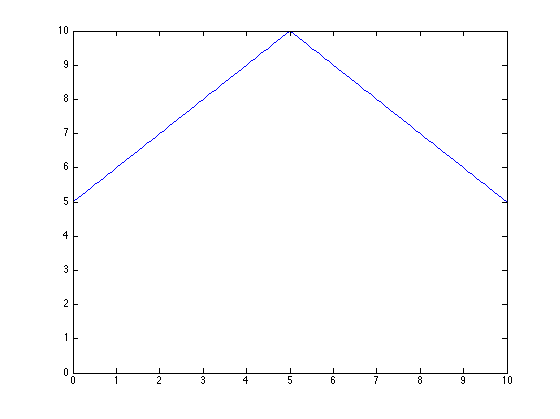
\includegraphics[scale = .5]{house.png}

By multiplying this matrix by a sheer matrix
\[ \left ( \begin{array}{cc}
1 & 1 \\
0 & 1 \end{array} \right) \]

we get a picture that looks like

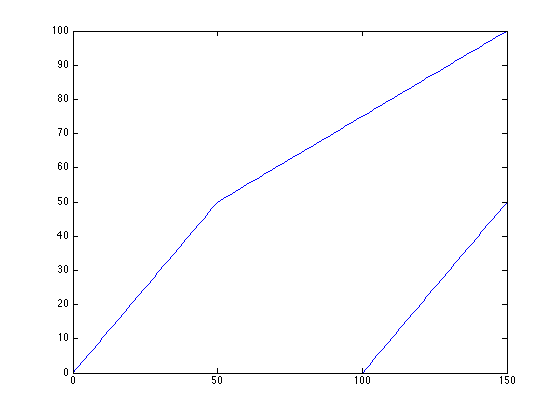
\includegraphics[scale=.5]{house1.png}
Here we get an image that is stretched horizontally to the right, as we are now adding the x and y coordinates together.  And finally if we multiply it by 
\[ \left (\begin{array}{cc}
1 & 2 \\
0 & 1 \end{array} \right) \]

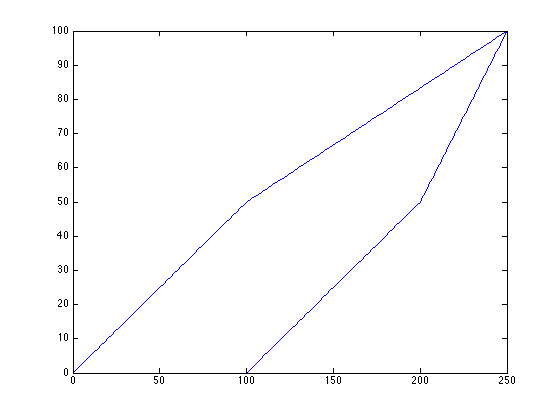
\includegraphics[scale = .5]{house2.png}
Similar to the other image, only we have doubled the rate of horizontal stretch.

2)\\
The file created gives us matrix for positions:

\[ \left ( \begin{array}{cc}
38 & -11 \\
-163 & -51 \\
196 & -43 \\
-249 & -155 \\
149 & 7 \\
-253 & 9 \\
-105 & 254 \\
100 & 236 \\
 224 & 115 \\
-335 & -97 \\
344 & 249 \\
221 & 26 \end{array} \right ) \]

we can convert this to a homogeneous matrix by adding a column of 0's and transposing the matrix, such that it becomes

\[ a3 = a2^T =  \left ( \begin{array}{cccccccccccc}
38 & -168 & 196 & -249 & 149 & -235 & -105 & 100 & 224 & -335 & 334 & 221\\
-11 & -51 & -43 & -155 & 7 & 9 & 254 & 236 & 115 & -97 & 249 & 26 \\
1 & 1 & 1 & 1 & 1 & 1 & 1 & 1 & 1 & 1 & 1 & 1 \end{array} \right ) \] 

and a Homogenous transform matrix

\[ HC = \left( \begin{array}{ccc}
1 & 0 & 300\\
0 & 1 & 300\\
0 & 0 & 1\end{array} \right ) \]

By multiplying these matrices together we get
\[ HC * a3  = \left ( \begin{array}{ccc}
338 & 137 &...\\
289 &  249 &...\\
1 &  1 &... \end{array} \right ) \]


by transposing this matrix and removing the 3rd column, we have a matrix that can easily be fed into matlab to get an image such as:

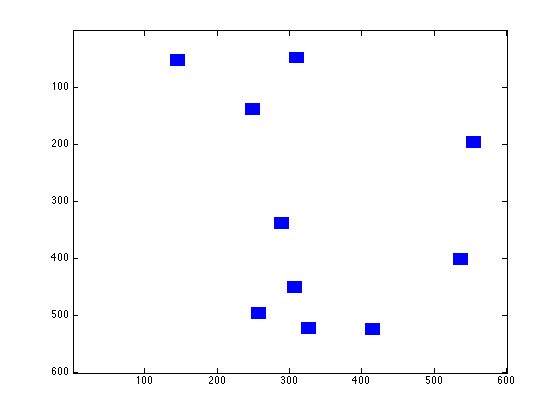
\includegraphics[scale=.5]{q2_2.png}

3)\\
A matrix that homogeneous and scales the X direction by 3/5 and Y direction by 5/4 looks like

\[ \left | \begin{array}{ccc}
3/5 & 0 & 0 \\
0 & 5/4 & 0 \\
0 & 0 & 1 \end{array} \right | \]

When this matrix is multiplied blocks that are graphed, you end up with a image that appears as

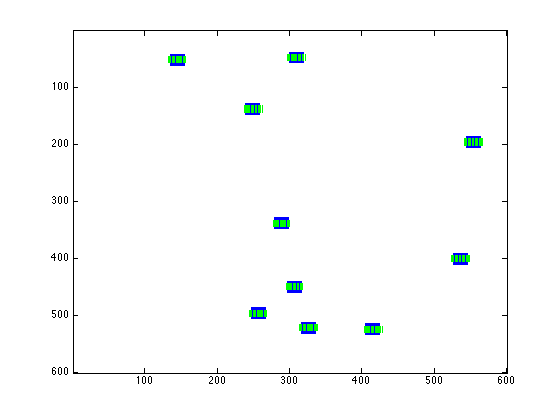
\includegraphics[scale=.5]{q3_1.png}

The next step requires to use of a rotation matrix which would appear as

\[ \left ( \begin{array}{ccc}
sin(\theta) & sin(\theta) & 0 \\
-sin(\theta) & sin(\theta) & 0\\
0 & 0 & 1 \end{array} \right ) \]

so in the case of rotating a matrix 30 degrees we end up with

\[ \left ( \begin{array}{ccc}
sin(30) & sin(30) & 0\\
-sin(30) & sin(30) & 0 \\
0 & 0 & 1 \end{array} \right ) 
 = 
 \left (\begin{array}{ccc}
 .5 & .5 & 0\\
 -.5 & .5 & 0\\
 0 & 0 & 1 \end{array} \right ) \]
 
 This matrix when multiplied against the previous matrix should result in an image as seen below.

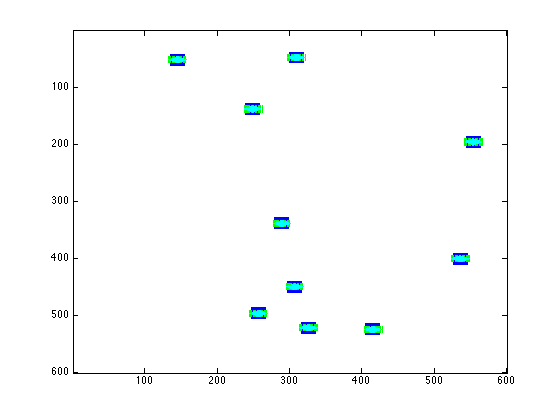
\includegraphics[scale=.5]{q3_2.png}

Finally a matrix to move each point (100,-200) looks like

\[ \left ( \begin{array}{ccc}
1 & 0 & 100\\
0 & 1 & -200\\
0 & 0 & 1\end{array} \right ) \]

all together a  matrix that would perform all those moves would look like

\[ \left ( \begin{array}{ccc}
0.3 & 0.3 & -30\\
-0.6 & 6.3 & -1312.5\\
0 & 0 & 1 \end{array} \right ) \]

a composite image off all these steps is seen in the last image.

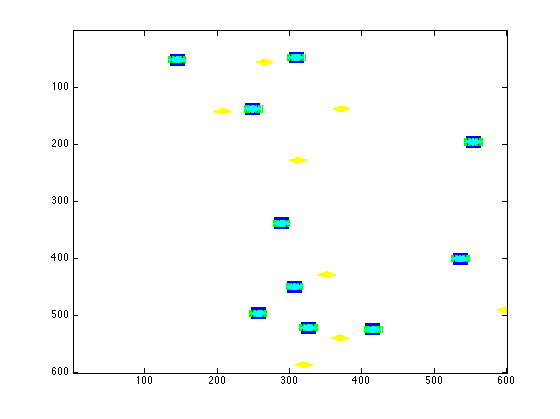
\includegraphics[scale=.5]{q3_3.png}


4)\\
5)\\
6)\\
7)\\
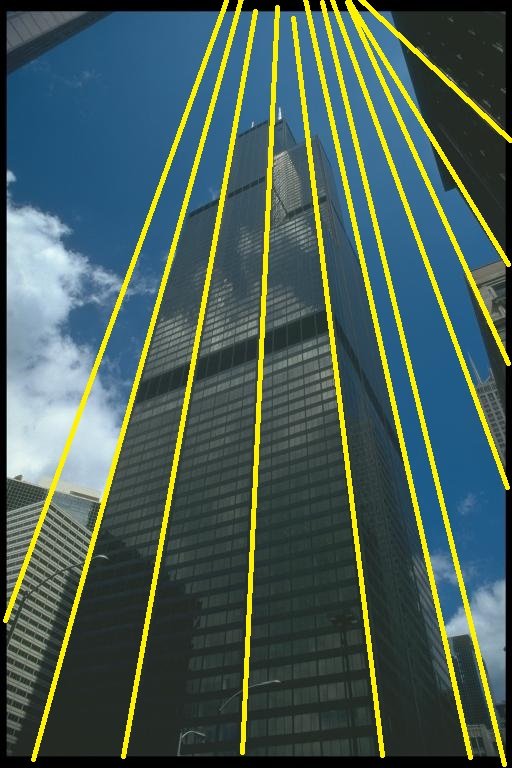
\includegraphics[scale=.5]{building.jpg}
For this image, you can basically see that the lines of the tower converge on a point somewhere high above is.  This is corroborated with the fact that the buildings on the edge of the frame are converging on the same focal point.  

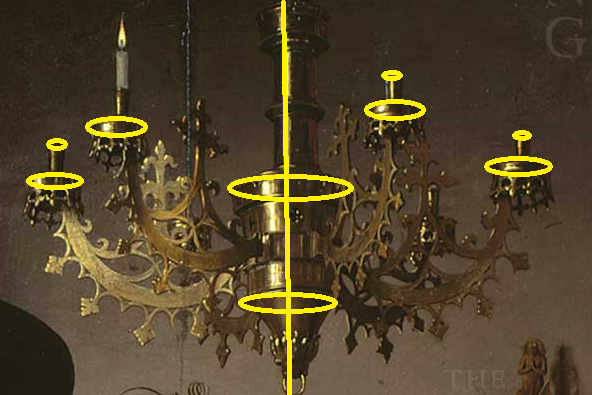
\includegraphics[scale=.5]{chandelier.png}\\
The difficulty with this image is that there is no hard line to infer a focal point.  I attempted to gain understanding of the focal point by estimating the angle at which the flat surfaces on top of the chandelier.  While it is not as concrete of a method as a straight line, with some calculation, we could figure out the angle at which this picture is taken to show a focal point.  





\end{document}